\documentclass[paper=a4, fontsize=11pt]{scrartcl} % A4 paper and 11pt font size

\usepackage[T1]{fontenc} % Use 8-bit encoding that has 256 glyphs
\usepackage{fourier} % Use the Adobe Utopia font for the document - comment this line to return to the LaTeX default
\usepackage[english]{babel} % English language/hyphenation
\usepackage{amsmath,amsfonts,amsthm} % Math packages
\usepackage{lipsum} % Used for inserting dummy 'Lorem ipsum' text into the template
\usepackage{graphicx}
\usepackage{sectsty} % Allows customizing section commands
\allsectionsfont{\centering \normalfont\scshape} % Make all sections centered, the default font and small caps
\usepackage[utf8]{inputenc} 
\usepackage{fancyhdr} % Custom headers and footers
\pagestyle{fancyplain} % Makes all pages in the document conform to the custom headers and footers
\fancyhead{} % No page header - if you want one, create it in the same way as the footers below
\fancyfoot[L]{} % Empty left footer
\fancyfoot[C]{} % Empty center footer
\fancyfoot[R]{\thepage} % Page numbering for right footer
\renewcommand{\headrulewidth}{0pt} % Remove header underlines
\renewcommand{\footrulewidth}{0pt} % Remove footer underlines
\setlength{\headheight}{13.6pt} % Customize the height of the header

\numberwithin{equation}{section} % Number equations within sections (i.e. 1.1, 1.2, 2.1, 2.2 instead of 1, 2, 3, 4)
\numberwithin{figure}{section} % Number figures within sections (i.e. 1.1, 1.2, 2.1, 2.2 instead of 1, 2, 3, 4)
\numberwithin{table}{section} % Number tables within sections (i.e. 1.1, 1.2, 2.1, 2.2 instead of 1, 2, 3, 4)

\setlength\parindent{0pt} % Removes all indentation from paragraphs - comment this line for an assignment with lots of text

%----------------------------------------------------------------------------------------
%	TITLE SECTION
%----------------------------------------------------------------------------------------

\newcommand{\horrule}[1]{\rule{\linewidth}{#1}} % Create horizontal rule command with 1 argument of height

\title{	
\normalfont \normalsize 
\textsc{Københavns Universitet, Datalogisk Institut} \\ [25pt] % Your university, school and/or department name(s)
\horrule{0.5pt} \\[0.4cm] % Thin top horizontal rule
\huge Ugeopgave 13 - Gruppeopgave \\ % The assignment title
\horrule{2pt} \\[0.5cm] % Thick bottom horizontal rule
}

\author{Allan Nielsen, Troels Thomsen, Troels Kamp Leskes} % Your name

\date{\normalsize\today} % Today's date or a custom date

\begin{document}

\maketitle % Print the title

\section*{Rapport}

\begin{figure}[h!]
  \centering
    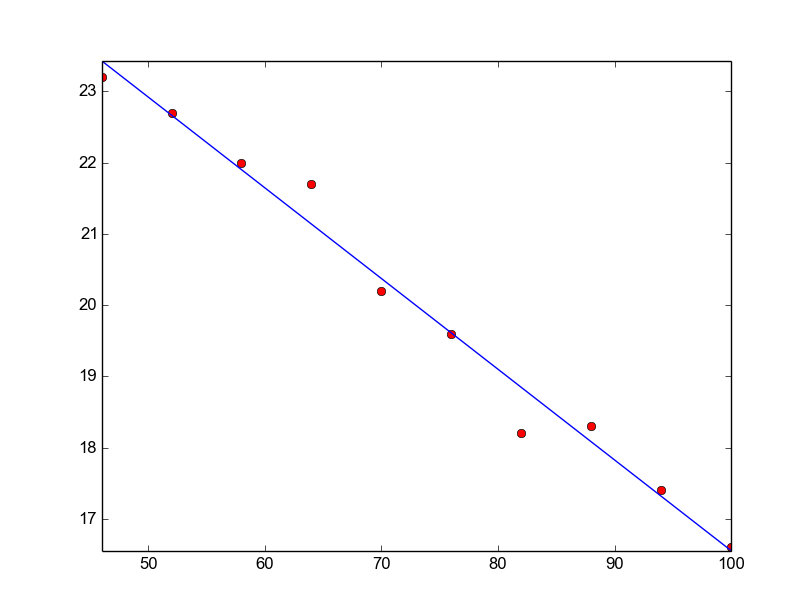
\includegraphics[width=.8\textwidth]{figure_1}
  \caption{over flueaeg med tilhørende regressionslinie}
\end{figure}
\pagebreak

Regressionslinien viser resultatet fra funktionen \textit{linearAnalysis()} anvendt på datasættet \textit{flueaeg.txt}. Figuren illustrerer hvordan den lineære analyse passer med datasættet ved at være indsat i samme figur. Figurens akser er generet ud fra \textit{(x min , x max ), (f (x min ), f (x max ))}
så samtlige punkter ingår i figuren. Regressionslinien passer ret præcist på punkterne, dermed er der en god sandsynlighed for at den er genereret korrekt. \\
For at kører testene skal filen \textit{RegressionTest.py} køres, for at vise figuren skal testfilen køres endnu en gang.\\

Ved at bruge xmin, xmax, fmin og fmax til afgrænsning af plottet, kan vi lave et mere dynamisk plot som er i stand til at tilpasse sig når dataene ændrer sig.\\

Vi har valgt at lave en hjælpefunktion regress i vores Regression klasse, som returnerer vores regressionsfunktion. Denne hjælpefunktion anvender vi til at finde punkterne på den linje vi gerne vil tegne i plottet.

\end{document}